%!TEX root=masterproef.tex

\chapter{Knoopverovering}
\label{appendix:node-capture}

Zoals reeds beschreven in de inleiding en in de situering hiervoorafgaand, is
de fysieke toegankelijkheid van knopen een re\"eel en groot probleem voor
draadloze sensornetwerken. In de volgende paragrafen illustreren we hoe
eenvoudig het is om een knoop te veroveren en dat de knoop en zijn netwerk hier
nagenoeg niets van kunnen merken.

\section{Situatie en doel}

Het hart van elke draadloze sensornetwerk knoop is de microcontroller of \mcu.
Door zijn ge\"integreerde architectuur bevat deze nagenoeg alle onderdelen die
interessant kunnen zijn en kan men zich louter hierop focussen bij een poging
om de knoop te veroveren.

In de testopstelling voor dit experiment maken we gebruik van een Atmel
ATMEGA1284p \citep{datasheet:atmega1284p}. Dit is een representatieve \mcu met
128KB programmeerbaar geheugen en 16KB werkgeheugen, die bv. gebruikt wordt in
de populaire Atmel RZRAVEN ontwikkelingskit \citep{manual:rzraven}. We kiezen
ervoor om de ATMEGA1284p volledig te ontdoen van enige context, om zo tevens de
algemeenheid van het probleem te illustreren.

De \mcu wordt voorzien van een eenvoudig programma dat een numerieke teller
verhoogt. Het doel van deze veroveringspoging is om de waarde van deze teller
te verkrijgen, zonder dat dit de werking van de \mcu verandert.

Figuur \ref{fig:node-capture-schematic} toont het schema van deze opstelling.

\begin{figure}[ht]
  \centering
  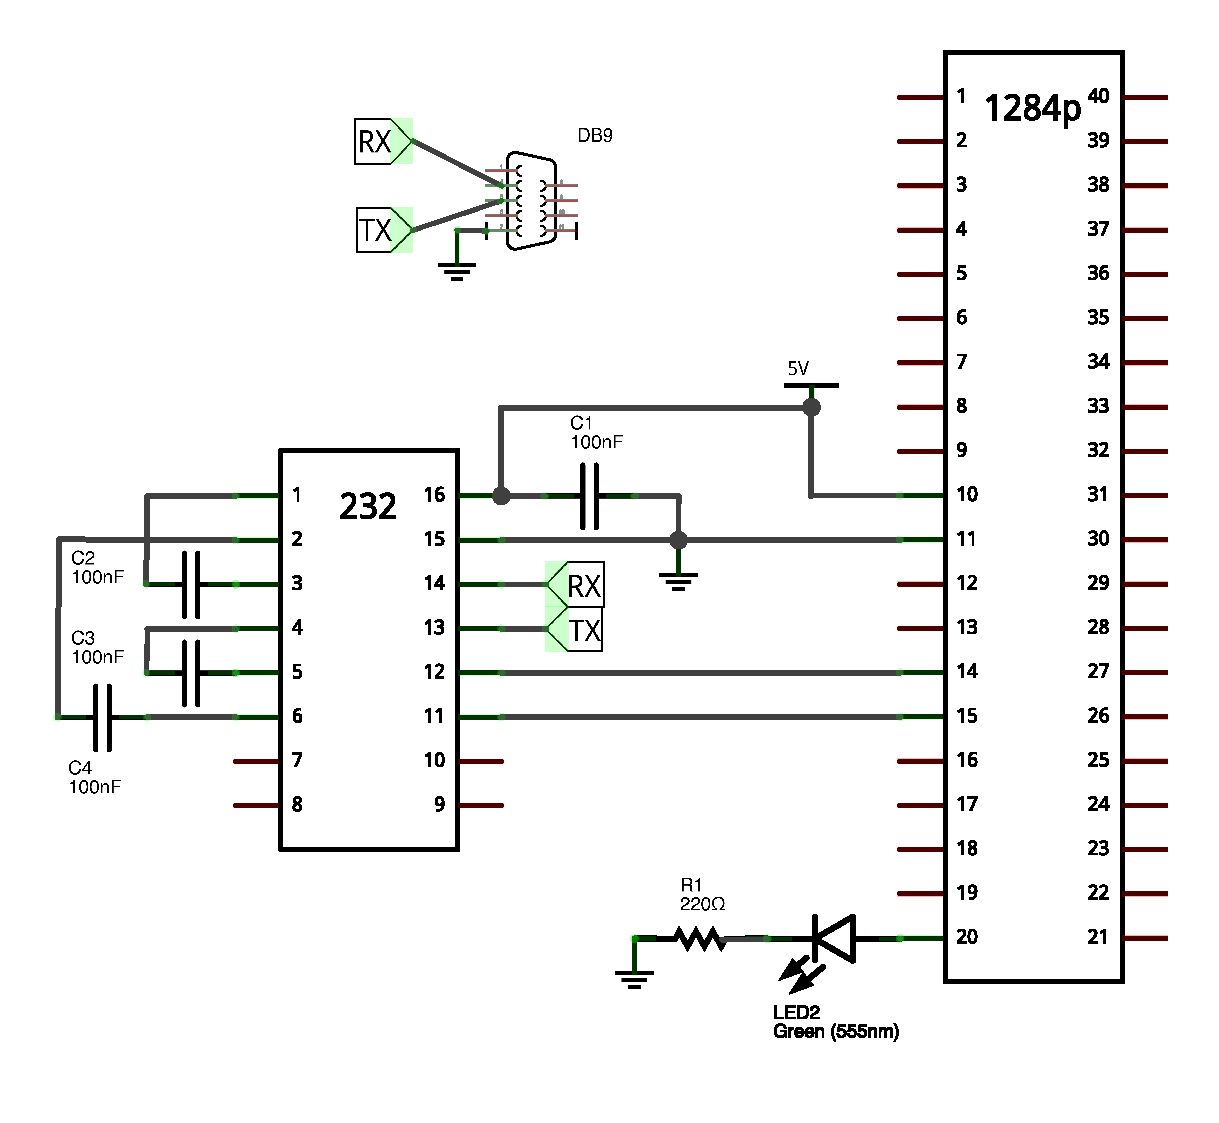
\includegraphics[width=0.7\linewidth]{resources/node-capture-schematic.pdf}
  \caption{Schema van de testopstelling voor knoopverovering.}
  \label{fig:node-capture-schematic}
\end{figure}

De \mcu is via een USART\footnote{USART staat voor \emph{Universal
synchronous/asynchronous receiver/transmitter} dat in staat voor de vertaling
van gegevens tussen een parallelle en seri\"ele voorstelling.} poort verbonden
met een MAX232 \citep{datasheet:max232} die de USART signalen omzet naar een
RS-232\footnote{RS-232 is een seri\"ele communicatiestandaard, typisch gebruikt
tussen computers en randapparatuur, maar ook kan dienen als eenvoudige data
verbinding tussen twee computers.} compatibele communicatie.

Codevoorbeeld \ref{lst:node-capture} toont de functionaliteit die op de \mcu
ge\"implementeerd werd: een globale variabele, \ttt{counter}, wordt eindeloos
verhoogd. Na elke verhoging wordt de waarde via de USART en de RS-232
verbinding naar een terminal verzonden. 

\inputminted[linenos,frame=lines,framesep=2mm,fontsize=\footnotesize]{c}{../src/node-capture/main.c}
\vspace{-5mm}
\captionof{listing}{Functionaliteit van de testopstelling voor knoopverovering.
  \label{lst:node-capture}}
\vspace{3mm}

Het is dus de bedoeling om de waarde van deze \ttt{counter} variabele te
bemachtigen, zonder dat de werking van het programma onderbroken wordt. Deze
variabele staat hier natuurlijk symbool voor eender welk gegeven dat in het
geheugen van de node wordt opgeslagen.

\section{Uitvoeren van de aanval}

De aanval bestaat er in dit geval in om de knoop te verbinden met een
hardwarematige foutopspoorder, zoals de Atmel JTAGICE mkII
\citep{manual:jtagicemkii}. Dit kan bv. gebeuren aan de hand van een JTAG
verbinding. Dit is een verbinding met tien draden, waarvan er vier aangesloten
moeten worden op de \mcu\footnote{Normaal gezien worden er 5 aangesloten. De
vijfde verbinding is de zgn. \ttt{RESET} aansturing. Aangezien we bij deze
aanval de \mcu zeker niet willen resetten, kan deze verbinding weggelaten
worden.} en twee naar een voeding en aarding geleid moeten worden. Zoals te
zien is op figuur \ref{fig:node-capture-jtag} worden de vier draden eenvoudig
op naast elkaar liggende pinnen (24 tot 27) van de \mcu aangesloten.

\begin{figure}[ht]
  \centering
  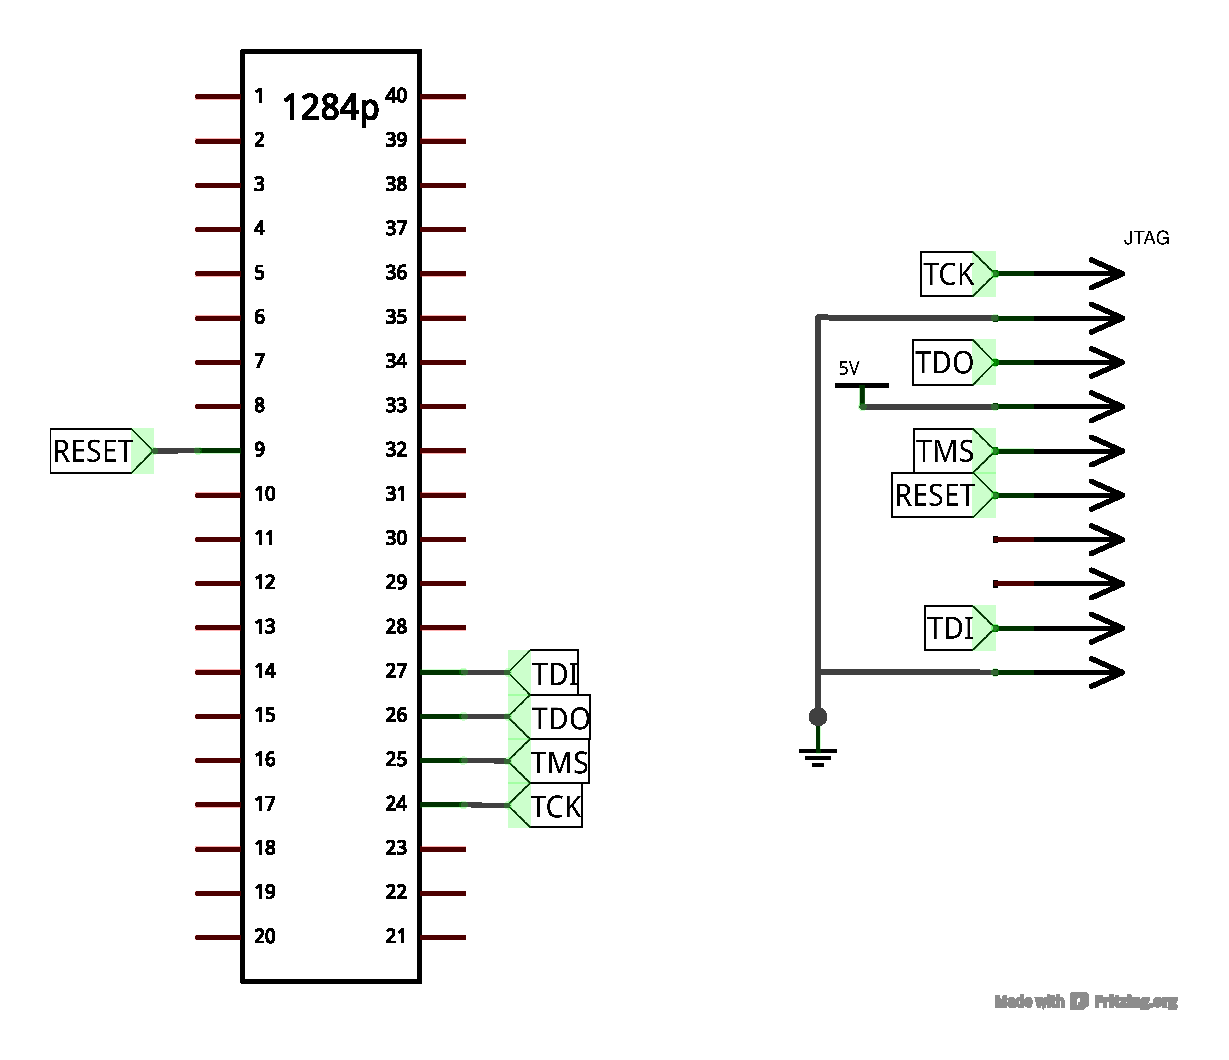
\includegraphics[width=0.7\linewidth]{resources/node-capture-jtag.pdf}
  \caption{Aansluiting van een JTAG verbinding.}
  \label{fig:node-capture-jtag}
\end{figure}

De uitvoer van de applicatie wordt weergegeven in listing
\ref{lst:node-capture-terminal} en toont een terminal applicatie die deze
uitvoer weergeeft. De applicatie werkt ononderbroken.

\begin{listing}[ht]
  \begin{minted}[linenos,frame=lines,framesep=2mm,fontsize=\footnotesize]{console}
$ screen /dev/tty.usbserial-FTSJ84AI 9600
counter = 1
counter = 2
...
counter = 10
counter = 11
counter = 12
counter = 13
counter = 14
counter = 15
counter = 16
...
\end{minted}
  \caption{Uitvoer van de applicatie op de \mcu.}
  \label{lst:node-capture-terminal}
\end{listing}

Tijdens dat deze uitvoer gerealiseerd werd, werd er echter een aanval
uitgevoerd. Deze werd gedaan aan de hand van de standaard
foutopsporingsmogelijkheden van de \mcu. Hiervoor werd een aangepaste versie
van de standaard foutopsporingssoftware
\ttt{gdb}\footnote{http://www.gnu.org/software/gdb/} gebruikt, nl.
\ttt{avr-gdb}.

Aangezien deze niet standaard met een JTAG verbinding kan werken, werd tevens
een brug opgezet door middel van
\ttt{avarice}\footnote{http://avarice.sourceforge.net}. Codevoorbeeld
\ref{lst:node-capture-avarice} toont het opstarten van de brug en het
beschikbaar maken van de JTAG verbinding via een locale server verbinding.

\begin{listing}[ht]
  \begin{minted}[linenos,frame=lines,framesep=2mm,fontsize=\footnotesize]{console}
$ avarice --mkII --capture --jtag usb:5a:cb :4242
AVaRICE version 2.13, Oct 29 2013 15:35:57

Defaulting JTAG bitrate to 250 kHz.

JTAG config starting.
...
Waiting for connection on port 4242.
Connection opened by host 127.0.0.1, port 58521.
  \end{minted}
  \vspace{-5mm}
  \caption{\ttt{avarice} brug tussen JTAG-gebaseerde foutopspoorder en \ttt{gdb}.}
  \label{lst:node-capture-avarice}
\end{listing}

Vervolgens kan de standaard foutopspoorder, \ttt{gdb}, gebruikt worden om het
geheugen van de \mcu te raadplegen en het programma verder te laten lopen.
Codevoorbeeld \ref{lst:node-capture-gdb} toont deze interactie.

\begin{listing}[ht]
  \begin{minted}[linenos,frame=lines,framesep=2mm,fontsize=\footnotesize]{console}
$ avr-gdb
GNU gdb 6.8
...
(gdb) target remote localhost:4242
Remote debugging using localhost:4242
0x000001d8 in ?? ()
(gdb) dump binary memory counter12.bin 8388892 8388900
(gdb) c
Continuing.
^C
Program received signal SIGINT, Interrupt.
0x000001d2 in ?? ()
(gdb) dump binary memory counter15.bin 8388892 8388900
(gdb) c
Continuing.
  \end{minted}
  \vspace{-5mm}
  \caption{\ttt{gdb} interactie met de \mcu.}
  \label{lst:node-capture-gdb}
\end{listing}

Codevoorbeeld \ref{lst:node-capture-hexdump} toont de inhoud van de veroverde
gegevens. \ttt{0c} en \ttt{0f} zijn telkens de eerste byte in het geheugen van
de \ttt{counter} variabele en tonen inderdaad de waarde die de variabele had op
het moment van de opvraging.

\begin{listing}[ht]
  \begin{minted}[linenos,frame=lines,framesep=2mm,fontsize=\footnotesize]{console}
$ hexdump counter12.bin 
0000000 0c 00 00 00 00 01 00 00                        
0000008

$ hexdump counter15.bin 
0000000 0f 00 00 00 00 01 00 00                        
0000008
  \end{minted}
  \vspace{-5mm}
  \caption{Interpretatie van de gedownloade geheugenplaatsen.}
  \label{lst:node-capture-hexdump}
\end{listing}

\section{Geheugens en geheugenplaatsen}

In de \ttt{gdb} sessie worden expliciete adressen in het geheugen gebruikt. Dit
was mogelijk mits enige voorkennis i.v.m. de gecompileerde code. De
\ttt{counter} variabele is een globale variabele en komt daarom terecht in de
\ttt{.bss} data sectie. Deze sectie heeft standaard een vaste plaats in het
data geheugen - dat bij de Harvard architectuur gescheiden is van het programma
geheugen \citep{avr-memory}. Figuur \ref{fig:avr-ram-map} geeft een overzicht
van de indeling van het data geheugen op een AVR \mcu.

\begin{figure}[ht]
  \centering
  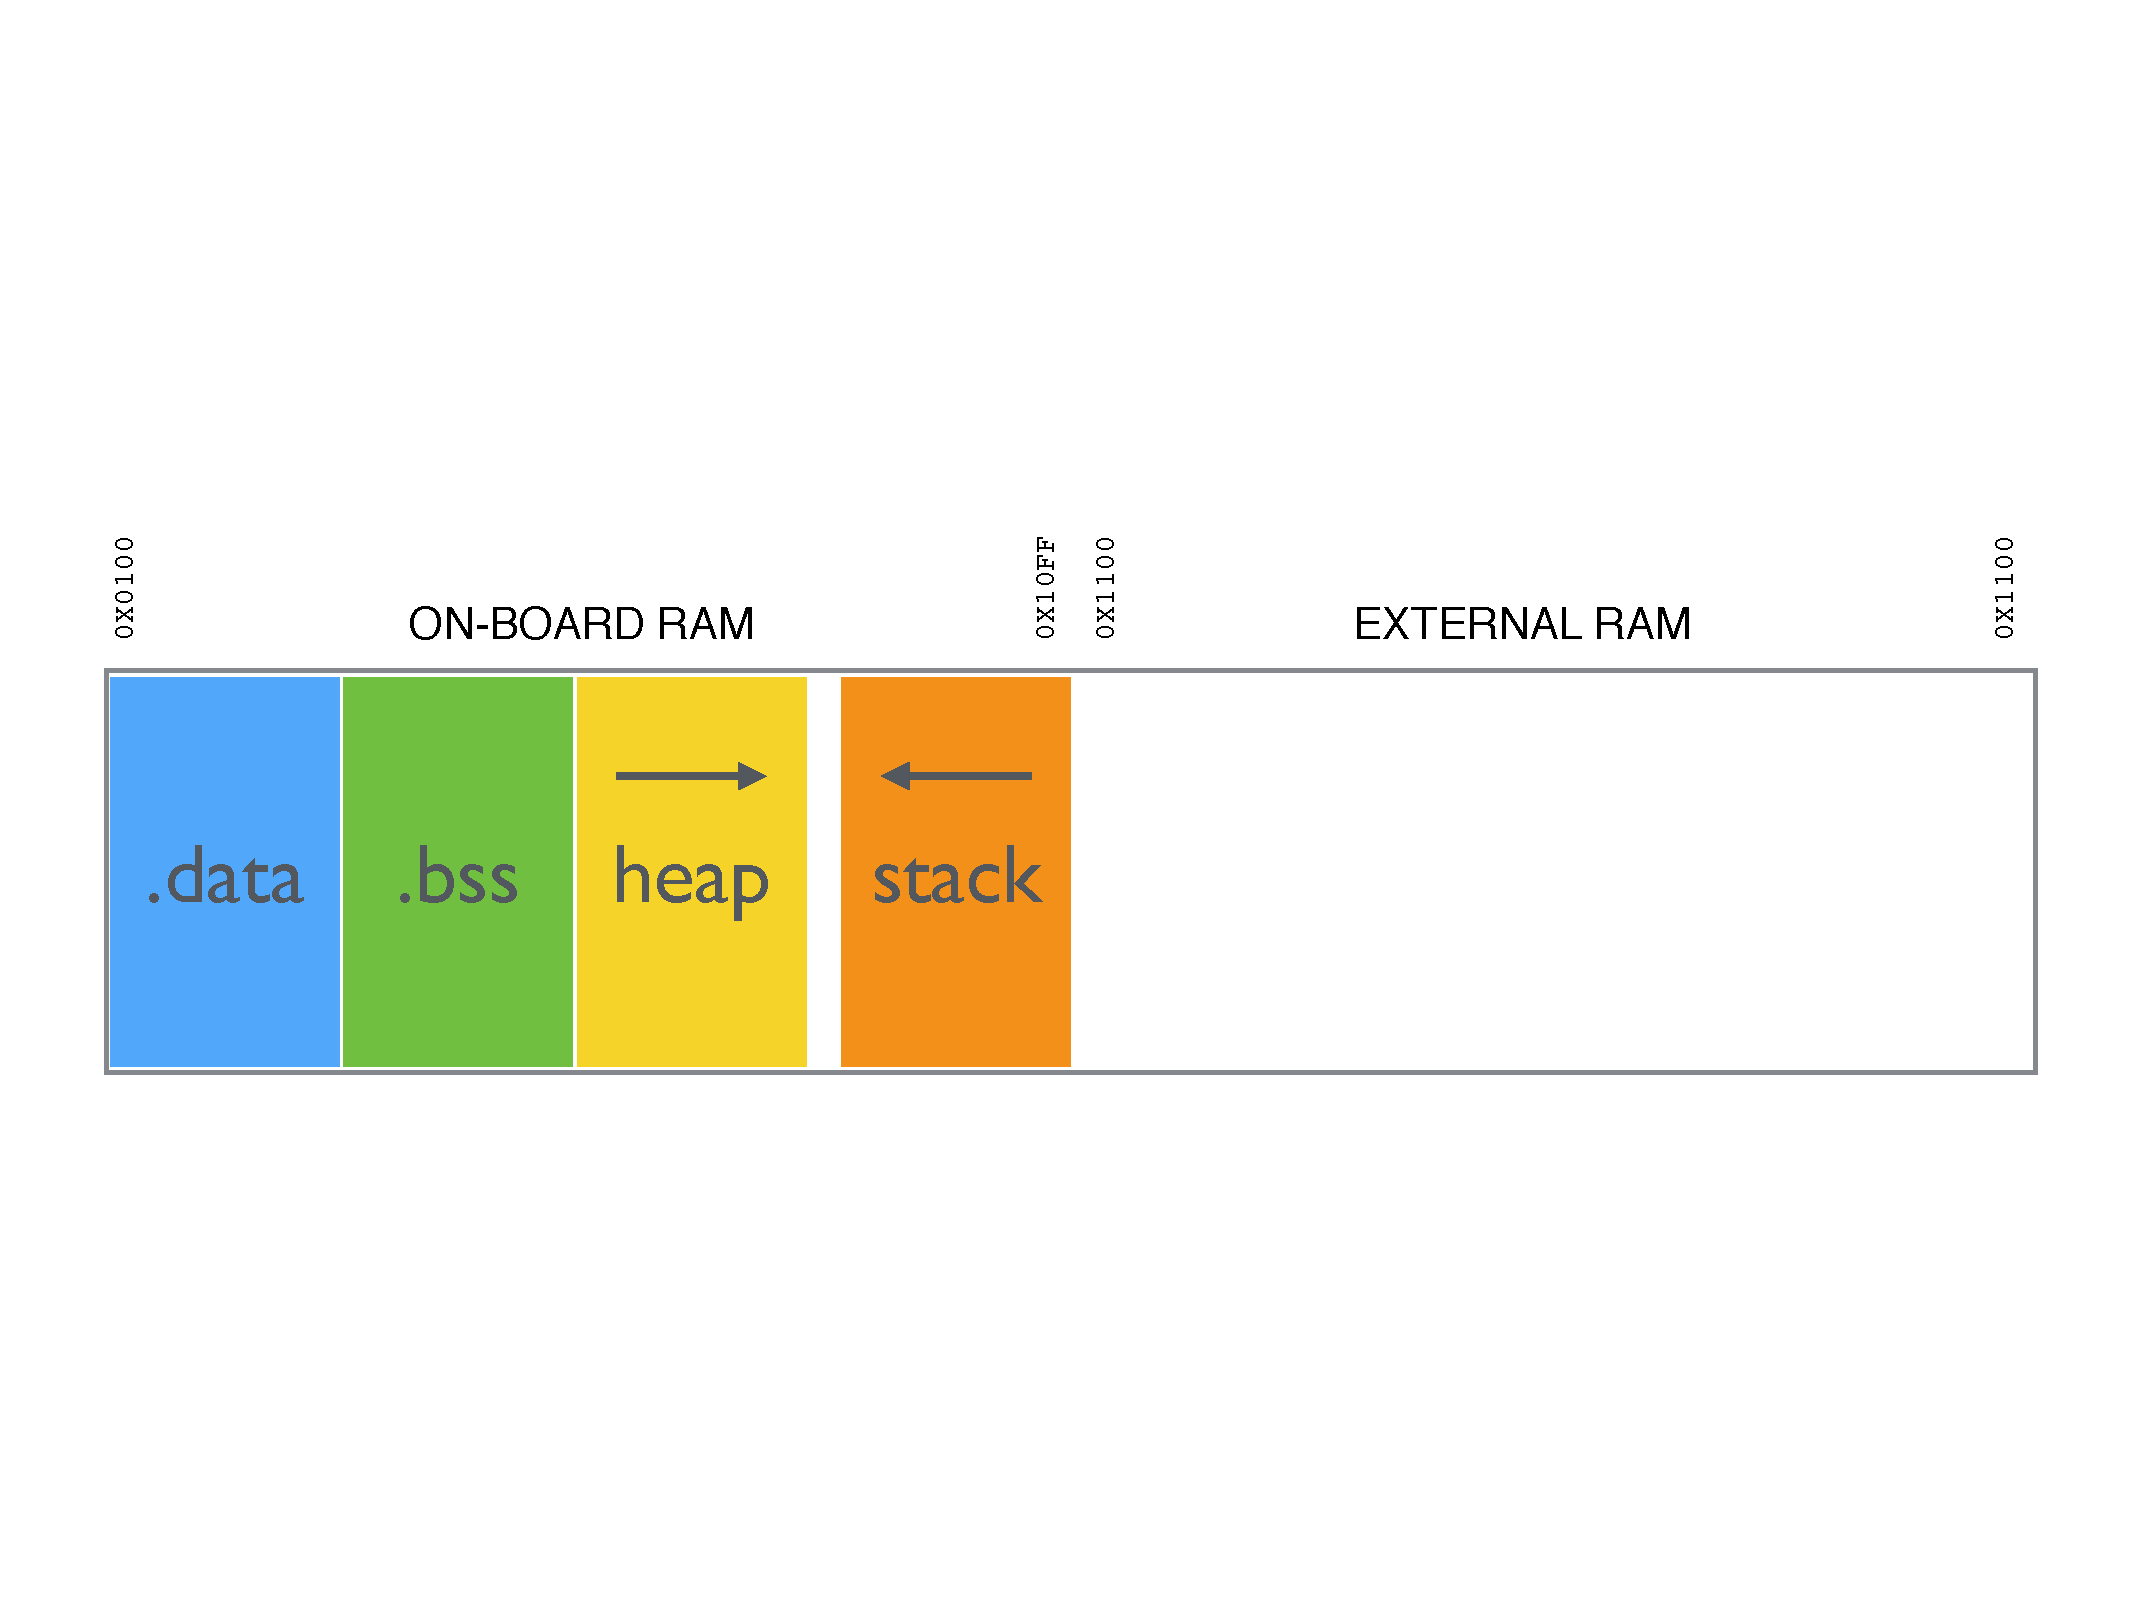
\includegraphics[width=0.9\linewidth]{resources/avr-ram-map.pdf}
  \caption{Indeling van het data geheugen \citep{avr-malloc}.}
  \label{fig:avr-ram-map}
\end{figure}

Zelfs zonder voorkennis over de code kunnen we het data geheugen benaderen. Het
binaire beeld dat naar de \mcu werd overgebracht, bestond uit de programma code
in de \ttt{.text} sectie en de \ttt{.data} sectie met de statische gegevens.
Aangezien de Harvard architectuur programma en data geheugen scheidt, wordt bij
het uitvoeren van het programma, de \ttt{.data} sectie gekopieerd naar dit
aparte data geheugen. Daarna wordt de \ttt{.bss} sectie gevuld en start de
opbouw van de \ttt{heap}.

We kunnen nu twee binaire beelden downloaden van de \mcu: het oorspronkelijk
ge\"uploade beeld en een kopie van het data geheugen. Dit laatste start op
adres \ttt{0x0100} met een bijkomende verschuiving van \ttt{0x800000}. Door het
einde van het oorspronkelijke beeld en het begin van het data geheugen te
vergelijken, kunnen we de \ttt{.data} sectie bepalen, als ook het begin van de
\ttt{.bss} sectie.

\section{Conclusies en gevolgen}

In bovenstaande paragrafen werd aan de hand van een beperkt voorbeeld
ge\"illustreerd hoe met standaard ontwikkelingsmiddelen, doelbewust het
geheugen van een werkende \mcu uitgelezen en ge\"interpreteerd kan worden.

Een eenvoudige variabele met een teller is zeker geen doelwit op zich, maar het
is denkbaar dat in een gelijkaardige globale variabele een encryptie sleutel,
of andere belangrijke informatie, opgeslagen wordt.

De mogelijkheid om via JTAG en OCD (On-Chip Debugging) het geheugen te
benaderen moet echter wel toegelaten worden door de instellingen van de \mcu.
Maar ook deze instellingen kunnen ook door kwaadwilligen aangepast worden, net
zoals door de rechtmatige eigenaar en ontwikkelaar van de knoop.

Het aanpassen van deze instellingen gaat echter gepaard met het herstarten van
de \mcu, omdat ze deel uitmaken van de programmatie. Indien de software van een
knoop dus bij het opstarten een validatie doet van de instellingen van de \mcu
kan het controleren dat deze instellingen geen kwaadaardige acties toelaten.
Indien wel, kunnen ze er voor zorgen dat ze geen belangrijke informatie
ontvangen van het netwerk en opslagen in het data geheugen.

Hieruit blijkt dat een minimaal onderdeel van een inbraakdetectiesysteem een
controle zal zijn van de instellingen van de \mcu, wat onderdeel kan uitmaken
van een globaal \emph{anomalie-detectie} subsysteem.
